\documentclass[tikz,border=3.14mm]{standalone}
\begin{document}
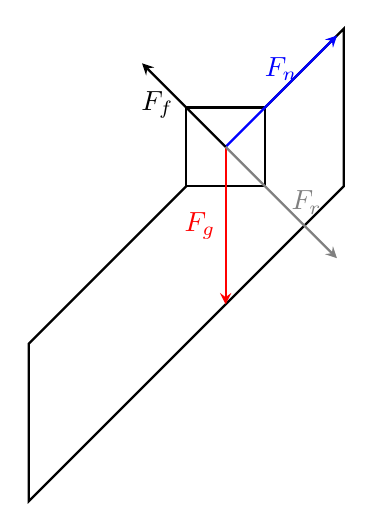
\begin{tikzpicture}[thick,>=stealth]
    % Draw the incline
    \draw (0,-2) -- (0,0) -- (4,4) -- (4,2) -- cycle;

    % Draw the cuboid at the middle of the incline
    \draw[fill=white] (2,2) rectangle +(1,1);
    \coordinate (center) at (2.5,2.5);

    % Draw and label the Forces
	% gravitational force
    \draw[->,red] (center) -- +(0,-2) node[midway,left] {$F_g$};
	% Normal Force
    \draw[->,blue] (center) -- +(45:2) node[midway,above] {$F_n$};
	% frictional force
    \draw[->,black] (center) -- +(135:1.5) node[midway,left] {$F_f$};
	% resulting force
    \draw[->,gray] (center) -- +(315:2) node[midway,right] {$F_r$};
\end{tikzpicture}
\end{document}